\section{Experiment Dashboard}
\label{sec:dashboard}

Managing a large-scale evaluation of Large Language Models (LLMs) for the Certified Reliability Engineer (CRE) exam presented significant operational challenges. With dozens of hyperparameters (temperature, RAG depth, model selection, few-shot constants) and hundreds of individual runs, our early development phase was hindered by "buried results" and the cognitive load of navigating raw JSON logs and configuration files. To solve this, we developed a centralized experiment dashboard using Streamlit (see Figure~\ref{fig:dashboard_interface}).

\begin{figure}[h]
    \centering
    \begin{minipage}{0.48\textwidth}
        \centering
        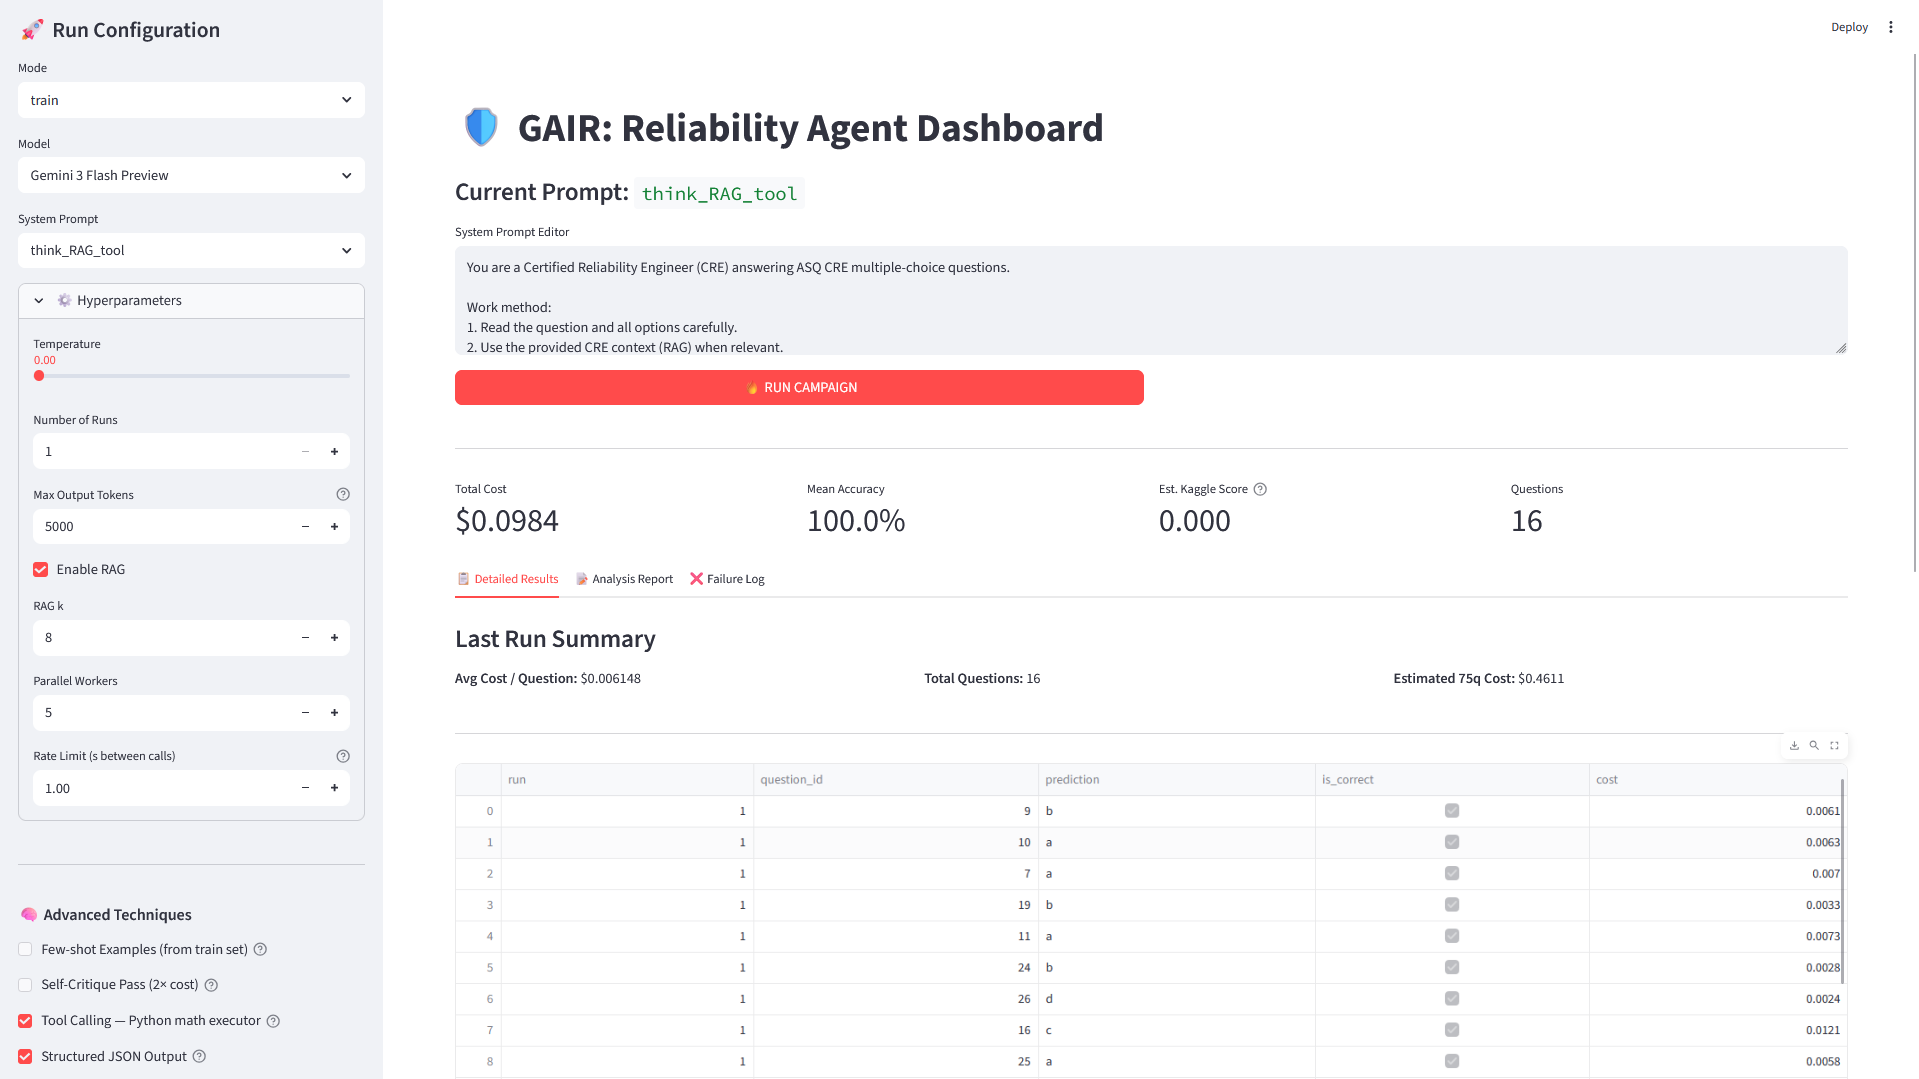
\includegraphics[width=\textwidth]{report/dashboard_config.png}
        \caption{Dashboard configuration sidebar for seamless parameter tuning.}
        \label{fig:dashboard_config}
    \end{minipage}
    \hfill
    \begin{minipage}{0.48\textwidth}
        \centering
        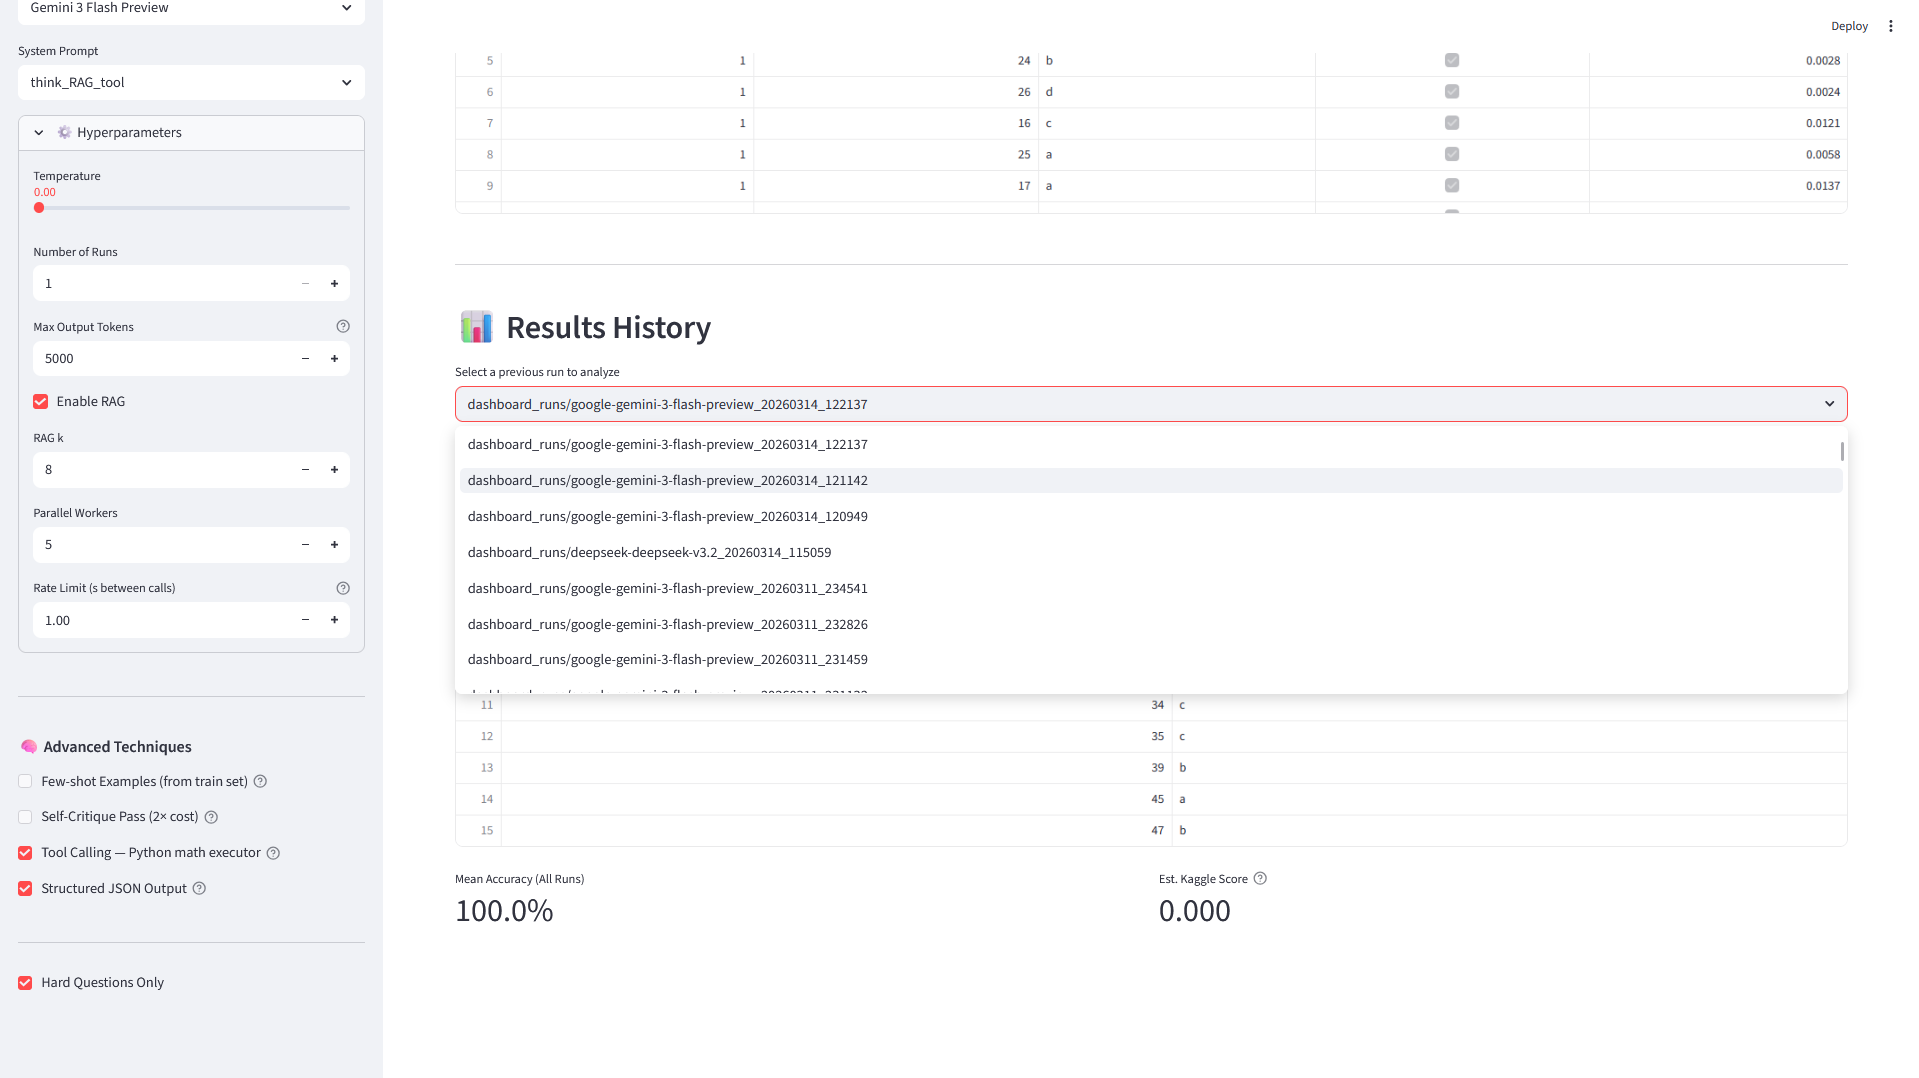
\includegraphics[width=\textwidth]{report/dashboard_runs.png}
        \caption{Real-time results tracking and historical run comparison.}
        \label{fig:dashboard_runs}
    \end{minipage}
\end{figure}

The dashboard addresses several primary pain points:
\begin{itemize}
    \item \textbf{Configuration Accessibility:} Instead of modifying hard-coded strings in deep nested scripts, users can select models (e.g., GPT-4o, Gemini 1.5 Pro), adjust temperatures, and toggle advanced reasoning techniques directly via a graphical interface. This allows team members to contribute to experiments without needing to understand the underlying implementation of the asynchronous runner or RAG pipeline.
    \item \textbf{No Source Code Dependency for Prompts:} Users no longer need to know where prompts are stored or how they are structured in the JSON backend. The dashboard provides a direct "System Prompt Editor" and prompt selection interface, abstracting away the file system.
    \item \textbf{Automated Chronological Logging:} Runs are automatically organized by timestamp and model name. The dashboard retrieves historical data (cost in USD, token usage, and accuracy) directly from the filesystem, providing a clear bird's-eye view of project progress over time.
    \item \textbf{Rapid Iteration on "Hard" Questions:} We implemented a specific toggle for "Hard Questions Only." This feature allowed us to instantly filter the dataset to 16 specific questions that were consistently failed by baseline models (e.g., Trinity). This targeted testing reduced the feedback loop from hours to minutes when testing new prompt engineering strategies.
\end{itemize}

Finally, the integration of a parallel worker setting in the sidebar was critical for efficiency. By allowing the configuration of up to 20 parallel workers with customizable rate limiting, we could execute full 75-question benchmarks across 5 randomized runs in under two minutes, significantly accelerating our development cycle.

\section{Reliability Engineering Tools}
\label{sec:tools}

Early error analysis revealed that while LLMs possess vast theoretical knowledge of reliability engineering, they consistently fail at multi-step numerical computations. Complex calculations involving the Weibull distribution, Poisson processes, or Chi-squared confidence intervals often resulted in "mental math" hallucinations, where the model's logic was correct but the arithmetic was flawed.

To bridge this gap, we implemented an agentic tool-calling loop centered around a \texttt{execute\_python\_math} tool.

\subsection{Python Math Executor}
Rather than relying on the LLM's internal weights for arithmetic, we provided the agent with a sandboxed Python environment. When the agent detects numerical data or keywords such as "MTBF," "Exponential," or "F-distribution," it is instructed to generate a Python script using libraries like \texttt{scipy.stats} and \texttt{numpy}. This script is executed in a secure subprocess, and the results are fed back into the model's context for final decision-making.

This tool was the single most impactful technical addition to our pipeline, facilitating a jump in accuracy from 86\% to 90\%. It ensured that the high-precision requirements of ASQ exams—where answers often differ only by a few decimal places—were met with computational rigor.

\subsection{Verifiability and Logging}
To ensure the reliability of the agent itself, we implemented detailed execution logs. These logs capture the exact code generated by the LLM, the raw output from the Python interpreter, and any execution errors.

\begin{figure}[h]
    \centering
    \begin{minipage}{0.95\textwidth}
        \small
        \begin{verbatim}
"tool_usage": [
  {
    "tool": "execute_python_math",
    "code": "import scipy.stats as stats\nimport math\n\n# Given data\nn = 10, mean_new = 0.86, std_new = 0.01, mu_old = 0.85\n# Calculate t-statistic for one-sample t-test\nt_stat = (mean_new - mu_old) / (std_new / math.sqrt(n))\ndf = n - 1\n# Critical t-value for two-tailed test (alpha = 0.05)\nt_crit_two = stats.t.ppf(1 - 0.05/2, df)\n# Confidence Interval calculation\nmargin_error = t_crit_two * (std_new / math.sqrt(n))\nci_lower = 0.86 - margin_error\nci_upper = 0.86 + margin_error\nprint(f\"{t_stat=}\")\nprint(f\"{ci_lower=}\")",
    "output": "t_stat=3.162277660168382\nci_lower=0.8528464309401166\nci_upper=0.8671535690598834"
  }
]
        \end{verbatim}
        \caption{Example of verified tool execution log for a statistical hypothesis testing question involving critical t-values and confidence intervals.}
        \label{fig:tool_logs_code}
    \end{minipage}
\end{figure}

The logging system allowed us to verify that the model was not only reaching the correct answer but was doing so for the right reasons. By inspecting the generated code, we could confirm that for complex statistical tasks, the model correctly utilized specialized functions (like \texttt{stats.t.ppf}) rather than attempting to estimate critical values from memory.
